\documentclass[]{article}
\usepackage{amssymb}
\usepackage{amsmath}
\usepackage[utf8]{inputenc}
\usepackage{graphicx}
\usepackage{booktabs}
\usepackage{listings}
\usepackage{color}
\usepackage{tabularx}
\usepackage{hyperref}

\definecolor{dkgreen}{rgb}{0,0.6,0}
\definecolor{gray}{rgb}{0.5,0.5,0.5}
\definecolor{mauve}{rgb}{0.58,0,0.82}

\lstset{frame=tb,
	%language=C++,
	aboveskip=3mm,
	belowskip=3mm,
	showstringspaces=false,
	columns=flexible,
	basicstyle={\small\ttfamily},
	numbers=none,
	numberstyle=\tiny\color{gray},
	keywordstyle=\color{blue},
	commentstyle=\color{dkgreen},
	stringstyle=\color{mauve},
	breaklines=false,
	breakatwhitespace=true,
	tabsize=2
}


\title{FYS4150 H20 - Project 4:\\The 2-Dimensional Ising Model and \\Monte Carlo Simulations}
\author{Olav Fønstelien}

\begin{document}
\maketitle

\begin{abstract}
%The abstract gives the reader a quick overview of what has been done and the most important results. Try to be to the point and state your main findings. It could be structured as follows 
% - Short introduction to topic and why its important 
% - Introduce a challenge or unresolved issue with the topic (that you will try to solve) 
% - What have you done to solve this 
% - Main Results 
% - The implications

This report gives presents a solution to the Ising model in two dimensions applied on a magnetic material. The model is interpreted as a reversible Markov process which we evolve using Monte Carlo simulation with the Metropolis algorithm as acceptance criteria. We give an outline of an efficient implementation of the model in a computer program, and show by simulation that the Markov process converges independently of initial state. The initial state may therefore be selected freely, with a relative cost or saving in equilibration time.

We use a $2 \times 2$ lattice to show that the model approximates the expectation values and variances of magnetic energy and moment with precision up to $10^{-3}$, but that this requires $\ge 10^6$ Monte Carlo cycles. We also show that the model can be used to estimate the lattice's energy probability distribution, and that it correctly reproduces the phase transition phenomena. The critical temperature of the infinite lattice, $T_C$, is approximated with an error of 0.31 \%.

Please visit my GitHub repository \url{https://github.com/fonstelien/FYS4150/tree/master/project4} for the source code developed for this report.

\end{abstract}

\section{Introduction} \label{sec:intro}
%When you write the introduction you could focus on the following aspects
% - Motivate the reader, the first part of the introduction gives always a motivation and tries to give the overarching ideas
% - What I have done
% - The structure of the report, how it is organized etc

The Ising model describes the binary magnetic orientation of the particles in a quadratic lattice. The state of each particle or \textit{spin} is either \textit{up} or \textit{down}, and the preferred state of each spin is to equal that of its four nearest neighbors. The ground state is up, and one could then maybe conclude that a lattice filled with ups makes for a dull model, but when applying an outer influence, like increasing the temperature, transitions away from the state of the neighbors become more likely. We would start to see areas of downs scattered in the lattice, a tendency which would only increase towards a complete random configuration as $T \rightarrow \infty$. 

In this report we will show how this evolution can be modeled as a Markov process. We will drive the process forward with the Monte Carlo method and pick spins from the lattice at random, which we then decide whether to flip or not -- \textit{yes} if the new state corresponds better to that of its neighbors; if not then \textit{maybe} -- to be decided by the Metropolis algorithm. We will see that this process, when repeated some hundred times over the lattice, makes the Markov process converge and the lattice reach its most likely state independently of its initial condition.

When the Markov process has converged, we will sample the magnetic energy and moment of the lattice and use these to derive statistical physical quantities -- heat capacity and magnetic susceptibility. We will also derive the probability distribution of the lattice energy at a given temperature, and show phase transitions in the material by changing the temperature and lattice extent. 

Even if an analytical solution to the two-dimensional Ising model exists, the model that we develop is easily extended to three or higher dimensions. The Ising model can also be used to describe other physical systems, or even to solve problems in the social sciences, where the \textit{state} of one individual is heavily influenced by the state of its nearest neighbors. As such, our study in this report could serve as an introduction to a more general method for solving problems of this nature.

We will start with a review of the mathematics needed to develop our model in Section \ref{sec:methods}, where we also give the outline of an efficient implementation in a computer program. Then we present results from the simulations of different lattice sizes and temperatures, including the effects of initial conditions, and an approximation of the probability distribution of the lattice energy in Section \ref{sec:results}. We end by summarizing our findings and drawing conclusions with some thoughts about future work in Section \ref{sec:conclusion}.

% MORE ABOUT THE REPORT STRUCTURE!


\section{Methods} \label{sec:methods}
% - Describe the methods and algorithms
% - You need to explain how you implemented the methods and also say something about the structure of your algorithm and present some parts of your code
% - You should plug in some calculations to demonstrate your code, such as selected runs used to validate and verify your results. The latter is extremely important!! A reader needs to understand that your code reproduces selected benchmarks and reproduces previous results, either numerical and/or well-known closed form expressions.

% L=2. Find the analytical expression for the partition function and the corresponding expectations values for the energy E, the mean absolute value of the magnetic moment |M| (we will refer to this as the mean magnetization), the specific heat CV and the susceptibility χ as functions of T using periodic boundary conditions. These results will serve as benchmark calculations for our next steps. 

The magnetic energy of each spin in a lattice depends on its neighbors. In the Ising model, the total energy $E$ of a lattice $\mathcal{L}$ is given by
\begin{equation} \label{eq:e-sum}
	E = -J \sum_{\langle kl \rangle} s_k s_l,
\end{equation}
where the value of a spin is either $+1$ or $-1$, and $\langle kl \rangle$ denotes all neighboring pairs of spins $s_k, s_l$ in the lattice. $J$ is the coupling constant and tells how strong the interrelation between neighboring spins is. In this report we will assume that $J > 0$. The magnetic moment of the lattice is
\begin{equation} \label{eq:m-sum}
	\mathcal{M} = \sum_{k} s_k;
\end{equation}
a simple sum over all spins in the lattice.


If we now let the lattice $\mathcal{L}$ be quadratic with $L \times L$ spins, the likelihood of any spin configuration $\mathcal{L}_i$ at a temperature $T$ is given by the Boltzmann probability distribution as
\begin{equation} \label{eq:pi}
	P(\mathcal{L}_i) = P_i = \frac{e^{-\beta E_i}}{Z}, \quad \text{where} \quad \beta = \frac{1}{k_BT}.
\end{equation}
$E_i$ is $\mathcal{L}_i$'s magnetic energy in this configuration, as given by Equation (\ref{eq:e-sum}), and $Z$ is the partition function for the canonical ensemble (see \cite{fys4150-notes}). The partition function is defined as
\begin{equation} \label{eq:partition-function}
	Z(\beta) = \sum_{i=1}^{M} e^{-\beta E_i},
\end{equation}
where $M = 2^{L^2}$ and $i = 1,2,...,M$ denotes each of the possible configurations $\mathcal{L}_i$ that $\mathcal{L}$ may have.

We see from Equations (\ref{eq:e-sum}), (\ref{eq:pi}) that if we let -1 denote a spin's \textit{down} state and +1 denote its \textit{up} state, the most likely state will be all ups, since this gives the lowest energy and hence highest probability, and at absolute zero temperature, this is how $\mathcal{L}$ will remain. 

However, increasing temperature will make other states more likely. Increased kinetic energy will cause individual spins to flip, giving the lattice a new state $\mathcal{L}_j$ with energy $E_j$. This process can be described by a Markov chain
\begin{equation} \label{eq:markov-chain}
	\mathbf{w}_{t+1} = \mathbf{W} \mathbf{w}_{t},
\end{equation}
where $\mathbf{w}_t = \{w_i\} = \{P_i\}$ denotes $\cal{L}$'s (discrete) probability distribution at time $t$. $\mathbf{W} = \{W_{i \rightarrow j}\}$ denotes the transition probabilities for all possible transitions $\mathcal{L}_i \rightarrow \mathcal{L}_j$, and is unknown. To overcome this, we will re-phrase $W_{i \rightarrow j}$ as a stochastic process, where the likelihood $T_{i \rightarrow j}$ of a spin to be a \textit{candidate} for the flip is equal for all, and the likelihood that we \textit{accept} this spin to flip is $A_{i \rightarrow j}$. That is;
\begin{equation}
	W_{i \rightarrow j} = T_{i \rightarrow j} A_{i \rightarrow j}.
\end{equation}

The Markov process is reversible and transition the other way, $\mathcal{L}_j \rightarrow \mathcal{L}_i$, is also allowed. We let $W_{j \rightarrow i} = T_{j \rightarrow i} A_{j \rightarrow i}$ denote the reverse process, and by taking the right side of Equation (\ref{eq:markov-chain}) we get the so-called detailed balance;
\begin{equation}
	\frac{W_{i \rightarrow j}}{W_{j \rightarrow i}} 
	= \frac{T_{i \rightarrow j} A_{i \rightarrow j}}{T_{j \rightarrow i} A_{j \rightarrow i}} 
	= \frac{A_{i \rightarrow j}}{A_{j \rightarrow i}}
	= \frac{w_j}{w_i} = \frac{P_j}{P_i} = e^{-\beta \Delta E_{i \rightarrow j}}.
\end{equation}
Here, $\Delta E_{i \rightarrow j}$ denotes the change in energy between state $\mathcal{L}_i$ and $\mathcal{L}_j$, $\Delta E_{i \rightarrow j} = E_j - E_i$. 

We will use the Metropolis algorithm to establish the two unknowns $A_{i \rightarrow j}$ and $A_{j \rightarrow i}$. The Metropolis algorithm states that if $\Delta E_{i \rightarrow j} \le 0$, we flat out accept the transition, such that $A_{i \rightarrow j} = 1$. The likelihood that we accept the reverse then becomes $A_{j \rightarrow i} = e^{-\beta \Delta E_{j \rightarrow i}}$, which gives us the general form of the Metropolis algorithm;
\begin{equation} \label{eq:metropolis}
	A_{i \rightarrow j} = 
	\begin{cases}
	1 &\text{if} \quad \Delta E_{i \rightarrow j} \le 0 \\
	e^{-\beta \Delta E_{i \rightarrow j}} &\text{otherwise}
	\end{cases}.
\end{equation}

The decision whether to accept the flip or not is then made in another stochastic process. In each iteration we draw a new random  number $r_i \sim \mathcal{U}(0,1)$ and apply it to the Metropolis algorithm. The result of the Metropolis algorithm is then given as
\begin{equation} \label{eq:metropolis-accept-or-not}
\begin{aligned}
	r_i &< A_{i \rightarrow j} \rightarrow \text{accepted} \\
	r_i &\ge A_{i \rightarrow j} \rightarrow \text{not accepted} \\
\end{aligned} \quad.
\end{equation}

\vspace{5mm}

The transition probability $\mathbf{W}$ is a stochastic matrix, which means that it has a single largest eigenvalue $\lambda_{max} = \lambda_1 = 1$, and for the remaining we have $0 < \lambda_i < 1$ \cite{fys4150-notes}. If we let $\mathbf{v}_i$ denote the corresponding eigenvectors, we can write the initial probability distribution $\mathbf{w}_{0}$ as
\begin{equation} \label{eq:initial-state}
	\mathbf{w}_{0} = \sum_{i} \alpha_i \mathbf{v}_i.
\end{equation}
After the first iteration we get
\begin{equation}
	\mathbf{w}_{1} = \mathbf{W} \mathbf{w}_{0} = \sum_{i} \lambda_i \alpha_i \mathbf{v}_i,
\end{equation}
and if we continue to the $p$th iteration, $\mathbf{w}_{p} = \mathbf{W}^p \mathbf{w}_{0} = \sum_{i} \lambda_i^p \alpha_i \mathbf{v}_i$, it becomes obvious that we reach a limit where
\begin{equation}
	\mathbf{w}_{q} \approx \lambda_1^q \alpha_1 \mathbf{v}_1 = \alpha_1 \mathbf{v}_1.
\end{equation}
Since the sum of the probability distribution in $\mathbf{v}_1$ must be equal to 1, that is; $\sum_{i} P_i = 1$, we must have $\alpha_1 = 1$. We then get that
\begin{equation} \label{eq:steady-state}
	\mathbf{w}_{t} = \mathbf{v}_1, \quad \text{for} \quad t \ge q,
\end{equation}
which means that after sufficient iterations, the probability distribution vector $\mathbf{w}_{t}$ becomes independent on the initial conditions $\mathbf{w}_{0}$. $\mathbf{w}_{t}$ will reach $\mathbf{v}_1$, which is the Boltzmann probability distribution for the defined partition function $Z(\beta)$ \cite{newman1999monte}, a quantity depending on temperature and the lattice itself. This means that if we allow ourselves enough time, the initial configuration of $\mathcal{L}$ can be selected freely since its probability distribution is bound to reach its most likely state from any initial configuration.

\vspace{5mm}

From Equation (\ref{eq:metropolis}) we see that the Metropolis algorithm lets us simulate the spin distribution of the lattice without knowing the partition function $Z(\beta)$. Evaluating this is not complicated, but it would require us to sum over all the possible configurations $\mathcal{L}_i$ of the lattice. The number of configurations is given by $M = 2^{L^2}$; a factor which very quickly becomes unwieldy. However, to derive any useful quantities for the lattice at a given temperature, it would still be necessary do sum over all configurations, unfortunately.

The expected magnetic energy and moment of the lattice are given by the equations
\begin{equation}
\begin{aligned}
	\mathbb{E}(E) &= \sum_{i=1}^{M} E_i P_i  = \frac{1}{Z} \sum_{i=1}^{M} E_i e^{-\beta E_i} \\
	\mathbb{E}(\mathcal{M}) &= \sum_{i=1}^{M} \mathcal{M}_i P_i  = \frac{1}{Z} \sum_{i=1}^{M} \mathcal{M}_i e^{-\beta E_i}
\end{aligned},
\end{equation}
respectively. Further, the heat capacity $C_V$ and magnetic susceptibility $\chi$ are given by  
\begin{equation}
\begin{aligned}
	C_V &= \frac{\sigma^2_E}{k_B T^2} \\
	\chi &= \frac{\sigma^2_\mathcal{M}}{k_B T} \\
\end{aligned},
\end{equation}
where the variances $\sigma^2_E, \sigma^2_\mathcal{M}$ again are given by
\begin{equation}
\begin{aligned}
	\sigma^2_E &= \frac{1}{Z} \sum_{i=1}^{M} E^2_i e^{-\beta E_i} - \mathbb{E}^2(E) \\
	\sigma^2_\mathcal{M} &= \frac{1}{Z} \sum_{i=1}^{M} \mathcal{M}^2_i e^{-\beta E_i} - \mathbb{E}^2(\mathcal{M}) \\
\end{aligned}.
\end{equation}

We see that in addition to $Z$, summing over $M$ reappears in these equations. Our strategy will therefore be to use Monte Carlo simulation and approximate the expectation values and variances by \textit{sample means} and \textit{sample variances}. We will simulate the evolving configurations $\mathcal{L}_i$ of the lattice by the stochastic Markov process described in Equations (\ref{eq:markov-chain}) through (\ref{eq:metropolis}), then wait until it converges (Equation (\ref{eq:steady-state})), and start sample the lattice's energies and magnetic moments $E_i, \mathcal{M}_i$.

The general equations for sample mean $\bar{\mu}_X$ and variance $\bar{\sigma}^2_X$ by $N$ samples are given by
\begin{equation}
\begin{aligned}
	\bar{\mu}_X &= \frac{1}{N} \sum_{i=1}^{N} X_i \\
	\bar{\sigma}^2_X &= \frac{1}{N} \sum_{i=1}^{N} X^2_i - \bar{\mu}^2_X \\
\end{aligned},
\end{equation}
which have the limits $\bar{\mu}_X \rightarrow \mathbb{E}(X)$ when $N \rightarrow \infty$ \cite{fys-stk4155-notes}.

\vspace{5mm}

We will now study how to best implement our Monte Carlo simulation of the Ising model in a computer program. To get good approximations for the expectation values, we will need to do hundreds of thousands or even millions of spin flip tests on our lattice. That we develop efficient code is therefore a high priority.

Our lattice $\mathcal{L}$ has limited extension with $L \times L$ spins, and the first thing we need do is to define the boundary conditions. Since we wish to simulate as large lattices as possible, we will use so-called \textit{periodic} boundary conditions, where the spins on the lattice edges are imagined to neighbor on each other. See \cite{fys4150-notes}. This has the approximate effect of extending our $L \times L$ lattice to $(L+2) \times (L+2)$.

Next we randomly pick a candidate to flip among the spins in the lattice, say $s_k$. We use the Metropolis algorithm in Equation (\ref{eq:metropolis}) to decide whether the flip is accepted or not, based on the change $\Delta E_{i \rightarrow j}$ in the lattice's energy from state $\mathcal{L}_i$ to $\mathcal{L}_j$. The change in the lattice's energy is given by
\begin{equation} \label{eq:dE}
	\Delta E_{i \rightarrow j} = E_j - E_i = 2J s_k^{(i)} \sum_{\langle l \rangle} s_l,
\end{equation}
where $\langle l \rangle$ denotes $s_k$'s four neighbors and $s_k^{(i)}$ denotes its state in $\mathcal{L}_i$. We observe that the sum over $s_l$ can take only five different values, such that
\begin{equation}
	\Delta E_{i \rightarrow j} = \{-8J, -4J, 0, 4J, 8J \}.
\end{equation}

Consequently, the Metropolis algorithm acceptance criteria $A_{i \rightarrow j}$ in Equation (\ref{eq:metropolis}) can take only five corresponding values at a given temperature $T$;
\begin{equation} \label{eq:metropolis-acceptance}
	A_{i \rightarrow j} = \{ 1, 1, 1, e^{-4J \beta}, e^{-8J \beta} \}, \quad \text{where} \quad \beta = \frac{1}{k_BT}.
\end{equation}
Pre-calculating these values and keeping them in a lookup table before we start the Markov process thus saves the potentially expensive calculation of the exponential function during the Monte Carlo simulation.

Before we start the process we should also calculate the lattice's energy and magnetic moment in the initial condition, $E, \mathcal{M}$. Then, whenever a candidate is accepted, the change in energy and magnetic moment are accumulated. However, to avoid clogging the CPU pipeline with conditionals when we implement the Metropolis algorithm, we should use a facility that is available in many programming languages which is that boolean expressions return \lstinline|integer|s when they are evaluated; \lstinline|0| for a \lstinline|FALSE| expression and \lstinline|1| for a \lstinline|TRUE|. If we let $b$ denote the result of the Metropolis algorithm (accept/not accept), we get the update rules
\begin{equation}
\begin{aligned}
	s_k &\leftarrow s_k - 2bs_k \\
	\mathcal{M} &\leftarrow \mathcal{M} + 2bs_k^{(j)} \\
	E &\leftarrow E + 2bJ s_k^{(i)} \sum_{\langle l \rangle} s_l \\
\end{aligned}.
\end{equation}

\vspace{5mm}

Listing \ref{lst:ising} gives an outline of an algorithm for solving the Ising model in two dimensions. It is implemented as a Markov chain and runs a Monte Carlo simulation with the Metropolis algorithm as acceptance criteria. 

Note that we accumulate the absolute value \lstinline|Mabs| of the magnetic moment. The reason for this is that the model becomes unstable and may shift between positive and negative values close to the critical temperature. Note also that one Monte Carlo cycle is defined here as one sweep over the whole lattice, meaning that we do $L^2$ Metropolis spin flip tests per cycle. 

Before we start sampling magnetic energy and moment with \lstinline|Eacc|, \lstinline|E2acc|, \lstinline|Macc| and \lstinline|M2acc|, we must let the model reach its steady state (equilibration). This is handled by running a number of cycles defined by the \lstinline|equilibration_cycles| parameter. The number of cycles to run before equilibration depends on the size of the lattice, its initial and target temperatures, and also the sequence of numbers coming from the random number generator. It can only be determined by trial and error, but equilibration will generally be slower for a larger lattice, and for a larger difference in initial and target temperatures.

The equilibration process is a sequential process, but the sampling process can be parallelized without any influence on the results. It is important, however, that each process has its own random number generator to avoid oversamping.

\begin{lstlisting}[caption={Solving the Ising model in two dimensions with Monte Carlo simulation and the Metropolis algorithm to approximate the mean values and variances of the magnetic energy and moment. Note that we accumulate the absolute value of the magnetic moment.},label={lst:ising},escapeinside={@}{@}] [!h]
	// Declarations
	Tinit : "initial temperature of the lattice"
	T : "target temperature of the lattice"	
	lattice : "LxL 2D array containing the spins"
	wij : "pre-calculated lookup table with Metropolis acceptance limits"
	equilibration_cycles : "non-sampled thermalizing cycles"
	monte_carlo_cycles : "sampled cycles"
	E, Mabs : "Energy and absolute value of magnetic moment in the lattice"
	Eacc, Macc : "Accumulated energy and magn. moment for mean calculation"
	E2acc, M2acc : "Acc. energy and magn. moment squared for variance calc."
	
	// Initializing
	init_lattice(lattice, Tinit)  // gives some initial state to spins
	init_metropolis(wij, T)  // @Equation (\ref{eq:metropolis-acceptance})@
	
	// Monte Carlo
	// Thermalizing...
	FOR i = 1...equilibration_cycles DO
		FOR j = 1...L*L DO
			sk : "randomly drawn spin from the lattice"
			dE : "delta-energy for sk acc. to @Equation (\ref{eq:dE})@"
			b : "1 or 0 based on metropolis algorithm with dE, wij (@Equation (\ref{eq:metropolis-accept-or-not})@)"
			sk @$\leftarrow$@ sk - 2*b
		END FOR
	END FOR
	
	// Sampling energy and magnetic moment
	"Initialize E, Mabs"
	"Set Eacc, Macc, E2acc, M2acc to 0"
	"Parallelize FOR loop with individual RNGs; reduce Eacc, E2acc, etc"
	FOR i = 1...monte_carlo_cycles DO
		Eacc @$\leftarrow$@ Eacc + E
		E2acc @$\leftarrow$@ E2acc + E*E
		Macc @$\leftarrow$@ Macc + M
		M2acc @$\leftarrow$@ M2acc + M*M		
		FOR j = 1...L*L DO
			sk : "randomly drawn spin from the lattice"
			dE : "delta-energy for sk acc. to @Equation (\ref{eq:dE})@"
			b : "1 or 0 based on metropolis algorithm with dE, wij (@Equation (\ref{eq:metropolis-accept-or-not})@)"
			sk @$\leftarrow$@ sk - 2*b
			E @$\leftarrow$@ E + b*dE
			M @$\leftarrow$@ Mabs + 2*b*sk
		END FOR
	END FOR	
	
	// Expectation values
	Emean @$\leftarrow$@ Eacc / monte_carlo_cycles
	Mmean @$\leftarrow$@ Macc / monte_carlo_cycles

	// Variances
	Evar @$\leftarrow$@ E2acc / monte_carlo_cycles - Emean*Emean
	Mvar @$\leftarrow$@ M2acc / monte_carlo_cycles - Mmean*Mmean	
\end{lstlisting}




% Equations (13.6) and (13.7) of the lecture notes. Show that only five possible values of the energy differences ΔE are possible for the two-dimensional Ising model. Figure out how to encode efficiently the energy differences in the Boltzmann distribution. See the discussions in section 13.5 of the lecture notes. Why don't you need to calculate exp−ΔEβ each time you update the energy?


% Write now a code for the Ising model which computes the mean energy E, mean magnetization |M|, the specific heat CV and the susceptibility χ as functions of T using periodic boundary conditions



%\clearpage
\section{Results} \label{sec:results}
% - Present your results
% - Give a critical discussion of your work and place it in the correct context.
% - Relate your work to other calculations/studies
% - An eventual reader should be able to reproduce your calculations if she/he wants to do so. All input variables should be properly explained.
% - Make sure that figures and tables should contain enough information in their captions, axis labels etc so that an eventual reader can gain a first impression of your work by studying figures and tables only.

In this section we will present the numerical results of the simulation model outlined in Listing \ref{lst:ising}. We will first evaluate its correctness on a $2 \times 2$ lattice -- the most demanding there is. Due to its few fundamental states, it puts all of our assumptions about the Metropolis algorithm to the test. Likewise, it puts high demand on the degree of randomness of our random number generator, and challenges our boundary conditions, since all spins are at the lattice's edge. The $2 \times 2$ lattice also has the added benefit of easily attainable analytical expressions for the expectation values and variances which we can measure our numerical results against.

Then we move on to looking at the equilibration time on a larger $20 \times 20$ lattice, where we will also confirm the convergence of the Markov process. We will also use this lattice to approximate the energy probability distribution and see how this changes with temperature. 

Finally, we will run simulations over a continuous range of temperatures, with different lattice sizes, to observe phase transitions and to calculate from our numerical results the critical temperature of the infinite lattice.


\subsection{Evaluation of the Model} \label{sec:eval-model}
% for L=2 in the x and y directions. Compare your results with the expressions from a) for a temperature T=1.0 (in units of kT/J).How many Monte Carlo cycles do you need in order to achieve a good agreeement? 

The partition function $Z(\beta)$ is prohibitively expensive to calculate for any lattice of more than a few spins in each direction. But to evaluate the correctness of our model, we can let $L=2$, which leaves us with only $M = 2^4 = 16$ different configurations. As we see in Table \ref{tab:2x2-states}, they can be aggregated to six fundamental states.

\begin{table}[!h]
	\caption{Fundamental states of the $2 \times 2$ lattice.}
	\label{tab:2x2-states}
	\begin{center}
		\begin{tabular}{c|c|c|c}
			\toprule
			\# up spins 		& \# configs		& energy	& moment	\\
			\midrule
			4				& 1				& -8J		& 4			\\
			3				& 4				&  0		& 2			\\
			2				& 4				&  0		& 0			\\
			2				& 2				& +8J		& 0			\\
			1				& 4				&  0		& -2		\\
			0				& 1				& -8J		& -4		\\
			\bottomrule
		\end{tabular}
	\end{center}
\end{table}

We see from the table that when we calculate the partition function for the $2 \times 2$ lattice, only three fundamental states exist. The function becomes
\begin{equation}
	Z_{2 \times 2} (\beta) = 12 + 2e^{8J \beta} + 2e^{-8J \beta} = 12 + 4\cosh 8J\beta.
\end{equation}
For the magnetic energy the corresponding expectation value and variance become
\begin{equation} \label{eq:energy-analytical}
\begin{aligned}
	\mathbb{E}(E_{2 \times 2}) &= -\frac{32J}{Z_{2 \times 2}} \sinh 8J\beta \\
	C_{V, 2 \times 2} &= \frac{1}{k_B T^2} \bigg( \frac{256J}{Z_{2 \times 2}} \cosh 8J\beta - \mathbb{E}^2(E_{2 \times 2}) \bigg) \\
\end{aligned},
\end{equation} \label{eq:moment-analytical}
and likewise for the magnetic moment; 
\begin{equation}
\begin{aligned}
	\mathbb{E}(|\mathcal{M}_{2 \times 2}|) &= \frac{8J}{Z_{2 \times 2}} (2 + e^{8J\beta}) \\
	\chi_{2 \times 2} &= \frac{1}{k_B T} \bigg( \frac{32J}{Z_{2 \times 2}} (1 + e^{8J\beta}) - \mathbb{E}^2(|\mathcal{M}_{2 \times 2}|) \bigg) \\
\end{aligned}.
\end{equation}
Here, we state again that $\beta = \frac{1}{k_B T}$.

In Tables \ref{tab:2x2-e-vals} and \ref{tab:2x2-m-vals} we see the results of the simulations for temperature $T=1.0$ $J/k_B$ over the range $10^1$ to $10^9$ Monte Carlo cycles. We see that the model produces the expected values, but that we need to run up to $10^5$ cycles to get good estimates of the expectation values. For the variances, the energy variance error is only $8.3 \cdot 10^{-3}$ for $10^7$ cycles, while the magnetic moment variance error never improves beyond about $10^{-2}$ to $10^{-3}$, unless we run up to $10^9$ cycles. Figure \ref{fig:2x2} shows the evolution for the first $10^7$ cycles.


\begin{figure}[!h]
	\centering
	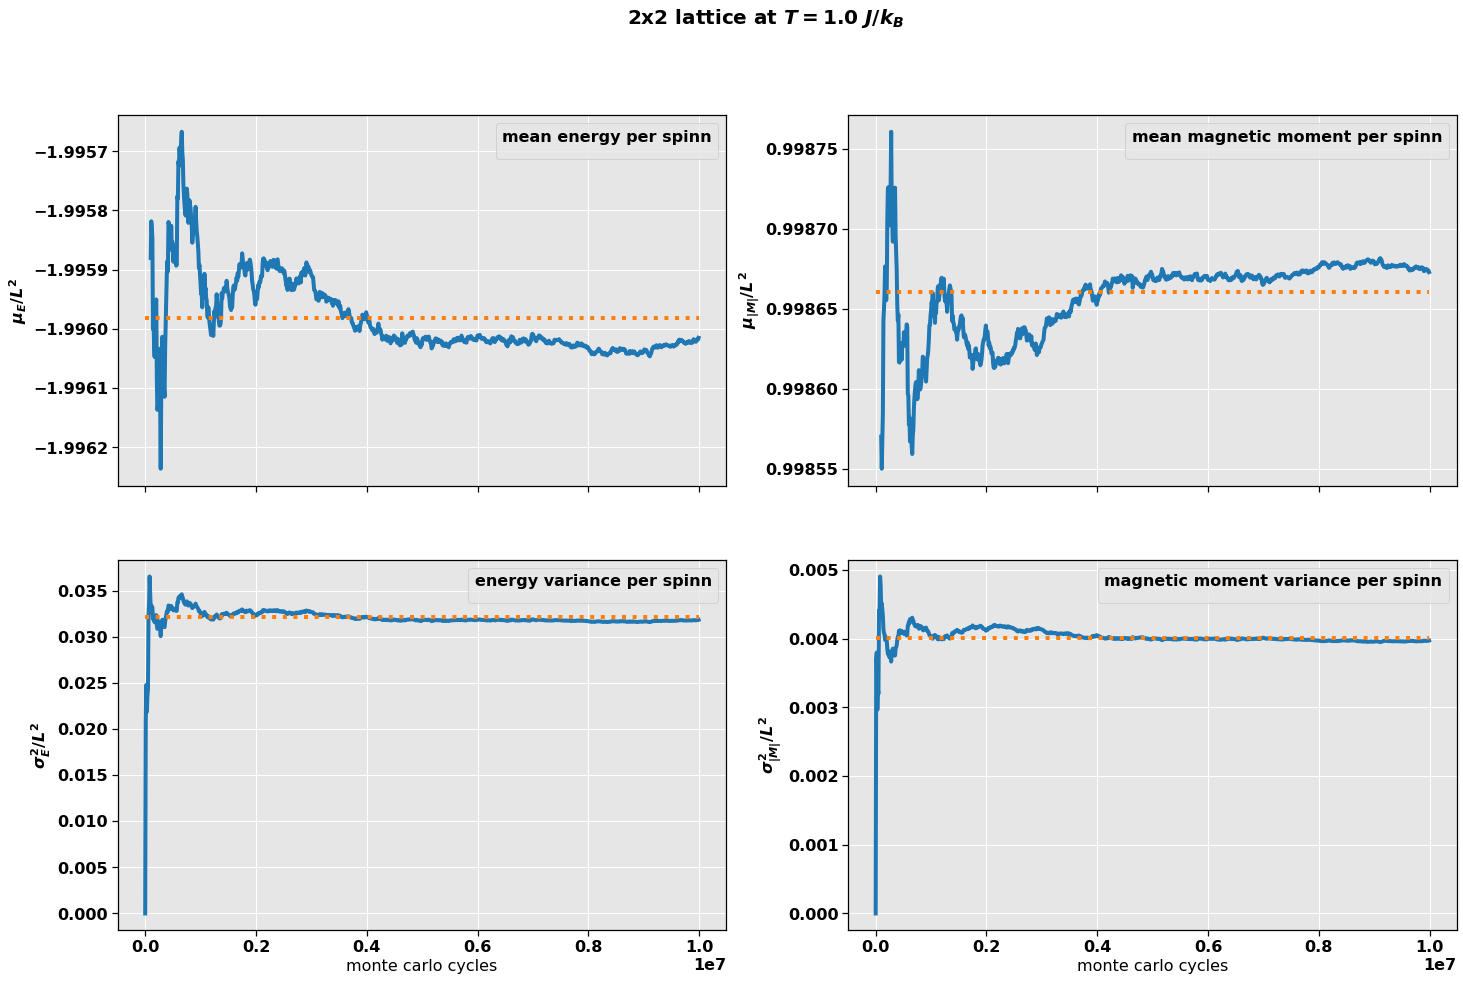
\includegraphics[width=1\linewidth]{./figs/2x2.png}
	\caption{Evolution of the mean values and variances for the first $10^7$ Monte Carlo cycles in a $2 \times 2$ lattice at $T = 1.0$ $J/k_B$. Note the differing scales. The dotted line indicates analytical values. Good agreement is reached after about $10^6$ cycles, but the relative error still remains in the $10^{-2}$ to $10^{-3}$ range for the variances. See Tables \ref{tab:2x2-e-vals} and \ref{tab:2x2-m-vals}.}
	\label{fig:2x2}
\end{figure}

\begin{table}[!h]
	\caption{Calculated energy for the $2 \times 2$ lattice at temperature $T=1.0$ $J/k_B$. We see that for the estimation of $\mathbb{E}(E)$, the error improves with a factor of about 10 up to $N = 10^5$, and a factor of 2 thereafter. For the estimation of $\sigma^2_E$, the error is about 100 times higher, and improvement is less for increasing $N$. True values are $\mathbb{E}(E) = -1.995982$ and $\sigma_E^2 = 3.208233 \cdot 10^{-2}$.}
	\label{tab:2x2-e-vals}
	\begin{center}
	\begin{tabular}{r|rr|rr}
		\toprule
		log$_{10}$ $N$ & $\bar{\mu}_E$ & $\varepsilon$ & $\bar{\sigma}^2_E$ & $\varepsilon$ \\
		\midrule
			1 & -1.81818e+00 & 8.90791e-02 & 1.32231e+00 & 4.02163e+01 \\
			2 & -1.98020e+00 & 7.90792e-03 & 1.56847e-01 & 3.88890e+00 \\
			3 & -1.99201e+00 & 1.99105e-03 & 6.36806e-02 & 9.84911e-01 \\
			4 & -1.99700e+00 & 5.10132e-04 & 2.39616e-02 & 2.53121e-01 \\
			5 & -1.99586e+00 & 6.11451e-05 & 3.30511e-02 & 3.01967e-02 \\
			6 & -1.99592e+00 & 3.01014e-05 & 3.25574e-02 & 1.48093e-02 \\
			7 & -1.99602e+00 & 1.67910e-05 & 3.18149e-02 & 8.33595e-03 \\
			8 & -1.99600e+00 & 7.17146e-06 & 3.19676e-02 & 3.57728e-03 \\
			9 & -1.99598e+00 & 2.39515e-07 & 3.20777e-02 & 1.42978e-04 \\
		\bottomrule
	\end{tabular}
	\end{center}
\end{table}

\begin{table}[!h]
	\caption{Calculated magnetic moment values for the $2 \times 2$ lattice at temperature $T=1.0$ $J/k_B$. The same observations for the mean value can be done here as for the energy mean value in Table \ref{tab:2x2-e-vals}. For the variance, however, the error seem to hit a limit at around $10^4$ cycles, and it seems to be unstable after that. True values are $\mathbb{E}(|\mathcal{M}|) = 0.9986607$ and $\sigma_{|\mathcal{M}|}^2 = 4.010740 \cdot 10^{-3}$.}
	\label{tab:2x2-m-vals}
	\begin{center}
		\begin{tabular}{r|rr|rr}
			\toprule
			log$_{10}$ $N$ & $\bar{\mu}_{|\mathcal{M}|}$ & $\varepsilon$ & $\bar{\sigma}^2_{|\mathcal{M}|}$ & $\varepsilon$ \\
			\midrule
				1 & 9.09091e-01 & 8.96899e-02 & 3.30579e-01 & 8.14233e+01 \\
				2 & 9.90099e-01 & 8.57320e-03 & 3.92118e-02 & 8.77671e+00 \\
				3 & 9.97003e-01 & 1.65996e-03 & 9.95408e-03 & 1.48186e+00 \\
				4 & 9.98800e-01 & 1.39574e-04 & 4.19382e-03 & 4.56479e-02 \\
				5 & 9.98560e-01 & 1.00853e-04 & 4.49166e-03 & 1.19908e-01 \\
				6 & 9.98648e-01 & 1.27485e-05 & 4.02668e-03 & 3.97554e-03 \\
				7 & 9.98673e-01 & 1.25342e-05 & 3.96926e-03 & 1.03425e-02 \\
				8 & 9.98666e-01 & 4.90383e-06 & 3.99568e-03 & 3.75535e-03 \\
				9 & 9.98661e-01 & 8.18624e-08 & 4.01068e-03 & 1.50076e-05 \\
			\bottomrule
		\end{tabular}
	\end{center}
\end{table}



\subsection{Equilibration Time} \label{sec:equilibration}
%  lattice with L=20 spins in the x and y directions

With the $2 \times 2$ lattice in the previous section, equilibration \textit{to} any temperature \textit{from} any temperature is a few cycles at most since the lattice will always be in one of the six possible fundamental configurations listed in Table \ref{tab:2x2-states}. A larger model, like the $20 \times 20$ that we will study here, allows for more configurations, and we therefore need to allow the model to reach equilibration before we can start sampling the magnetic energy and moment. Figure \ref{fig:20x20-wo-equilibration} clearly shows this. We see that starting at different configurations may bring some benefit -- especially for lower temperatures. At $T = 1.0$ $J/k_B$ all spins are usually up, corresponding well to the initial conditions. We also see that for this lattice, equilibration is reached at around 6000 cycles at the latest (lower right pane), but in reality sooner than that since the calculation of the average has a memory of the equilibration process.

\begin{figure}[!h]
	\centering
	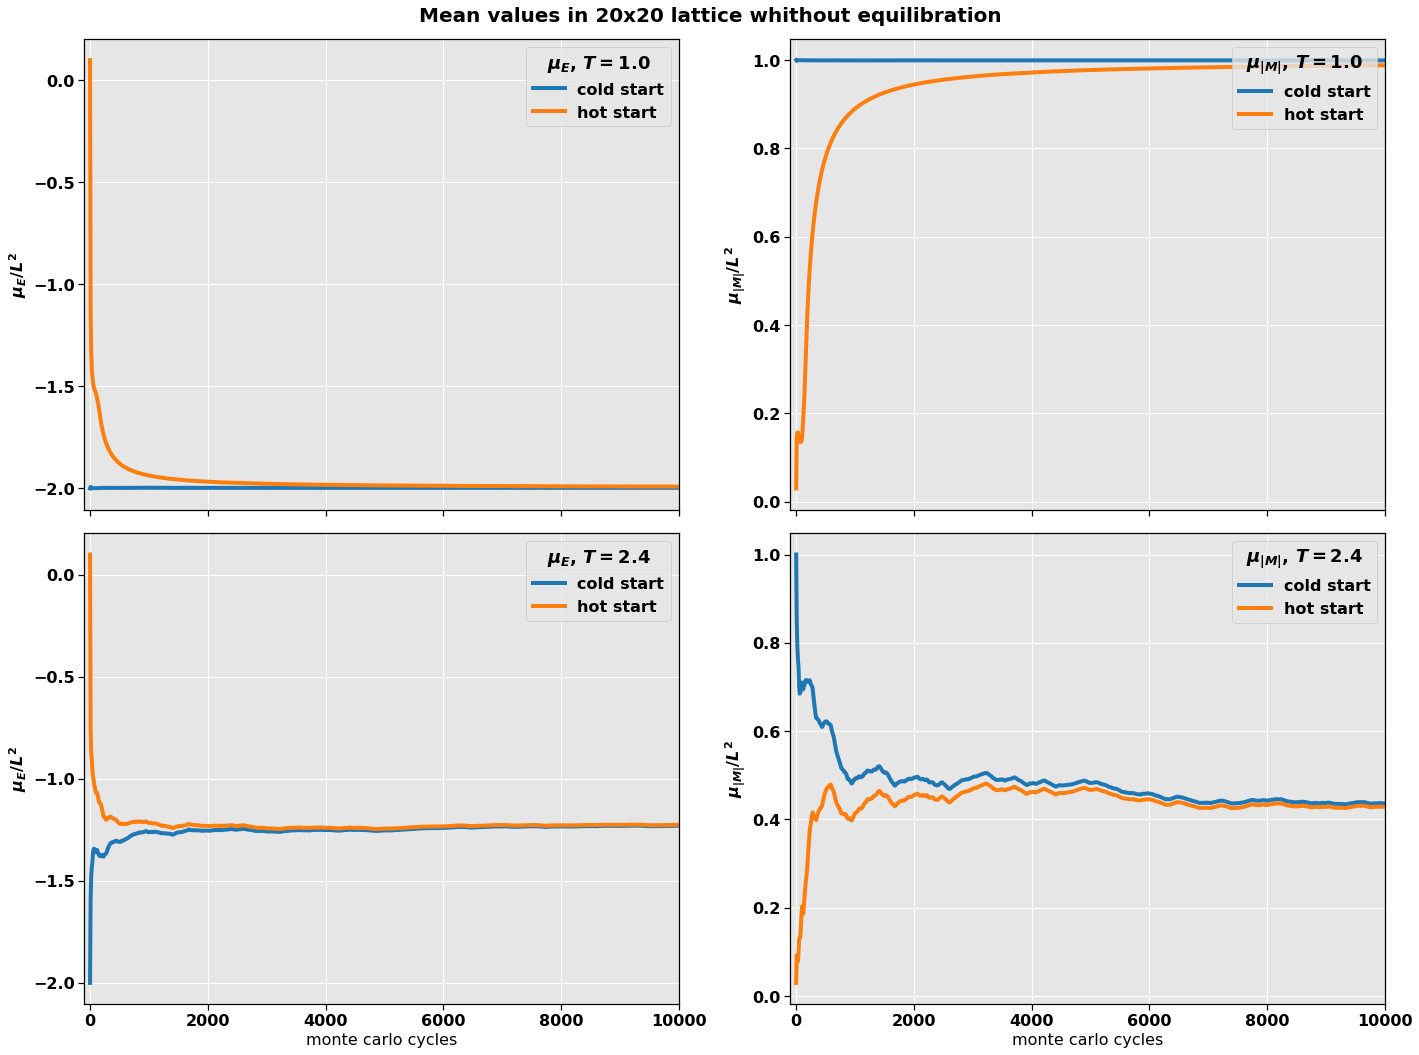
\includegraphics[width=1\linewidth]{./figs/20x20-wo-equilibration.png}
	\caption{Evolution of the mean values for the first $10^4$ Monte Carlo cycles in a $20 \times 20$ lattice at $T = 1.0$ $J/k_B$ in the upper panes, and $T = 2.4$ $J/k_B$ in the lower panes. We clearly see that we must allow some cycles for the model to reach equilibration, especially for higher temperatures. Cold start: all spins up; hot start; random spins. At $10^5$ cycles, and with equilibration, the estimated values are $\bar{\mu}_E = -1.997$ and $\bar{\mu}_{|\mathcal{M}|} = 0.9993$ per spin at $T = 1.0$ $J/k_B$; and $\bar{\mu}_E = -1.241$ and $\bar{\mu}_{|\mathcal{M}|} = 0.4632$ at $T = 2.4$ $J/k_B$.}
	\label{fig:20x20-wo-equilibration}
\end{figure}

Figure \ref{fig:20x20-config-energy} shows the evolution of the lattice energy $E_i$ in each configuration for the first 500 cycles. We see that the hot start energy confluences with the cold start energy as early as after 160-170 cycles for $T = 1.0$ $J/k_B$, and not very much later for $T = 2.4$ $J/k_B$. At this point the Markov process has converged. The probability distribution of the lattice has reached the Boltzmann distribution for the lattice at $T$, as shown in Equations (\ref{eq:initial-state}) to (\ref{eq:steady-state}). That is; $\mathbf{w}_t \rightarrow \mathbf{v}_1$. This becomes visible also when we look at the evolution of the number of accepted flips per Monte Carlo cycle in Figure \ref{fig:20x20-flips-per-cycle}; the hot start and cold start curves follow each other after confluence. Snapshots to confirm this are shown in Figure \ref{fig:20x20-config-spins}, where we see in the middle and right pane that the lattices match \textit{perfectly}. 

We should note that this result depends on that each process draws the same sequence of semi-random numbers from our random number generator, and may also be subject to the numerical precision in a CPU.

\begin{figure}[!h]
	\centering
	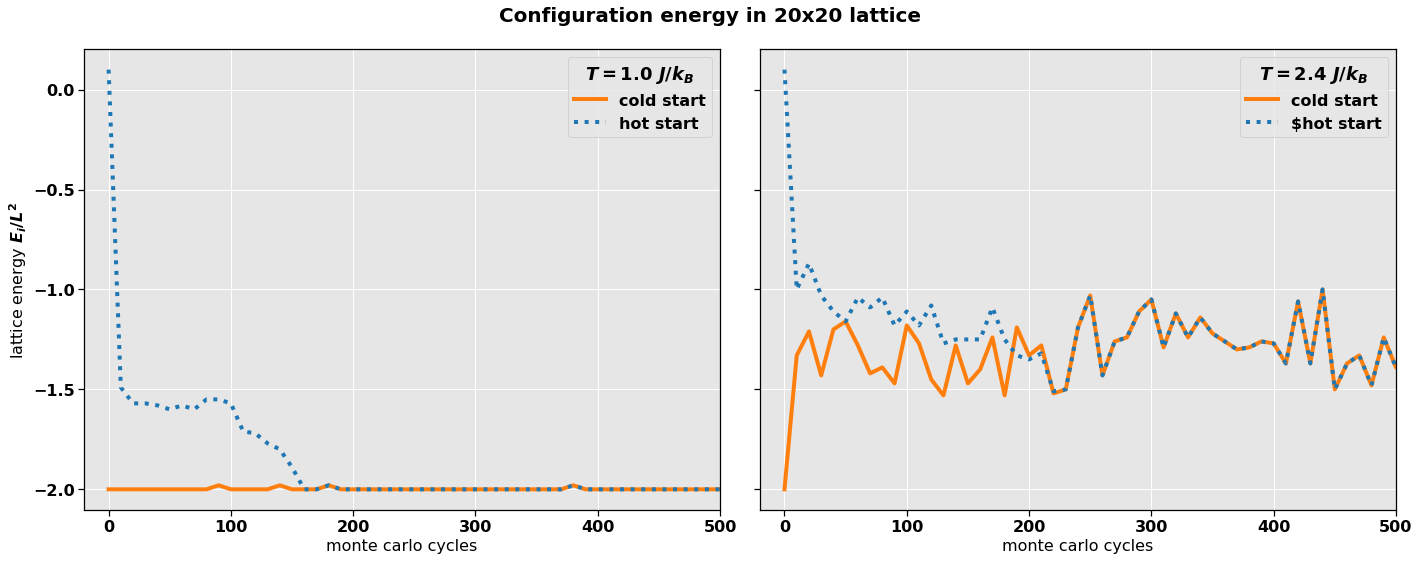
\includegraphics[width=1\linewidth]{./figs/20x20-config-energy.png}
	\caption{Evolution of the lattice energy $E_i$ in each configuration during the first 500 Monte Carlo cycles for a $20 \times 20$ lattice. The hot and cold start confluence at around 160 cycles for $T = 1.0$ $J/k_B$, and 200 for $T = 2.4$ $J/k_B$.}
	\label{fig:20x20-config-energy}
\end{figure}

\begin{figure}[!h]
	\centering
	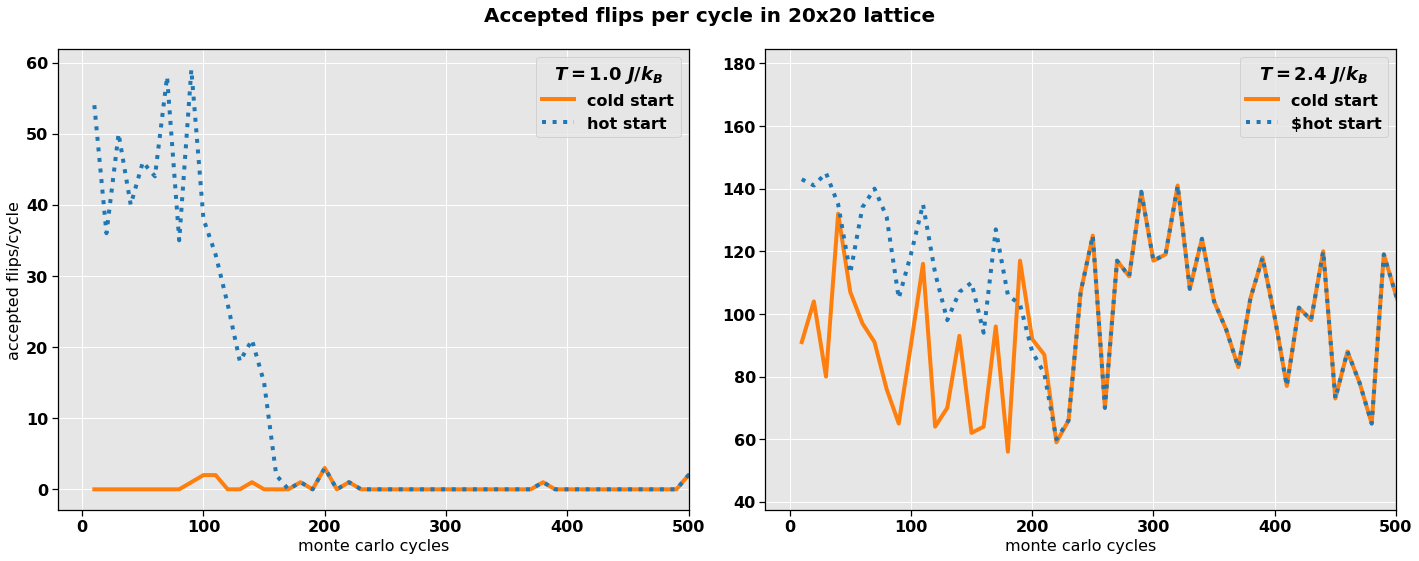
\includegraphics[width=1\linewidth]{./figs/20x20-flips-per-cycle.png}
	\caption{Accepted spin flips per Monte Carlo cycle during the first 500 Monte Carlo cycles for a $20 \times 20$ lattice. After confluence, the Markov process has converged and the evolution is independent of the lattice's initial configuration. Higher lattice temperature gives more accepted flips, as should be expected due to the higher kinetic energy of the spins.}
	\label{fig:20x20-flips-per-cycle}
\end{figure}

\begin{figure}[!h]
	\centering
	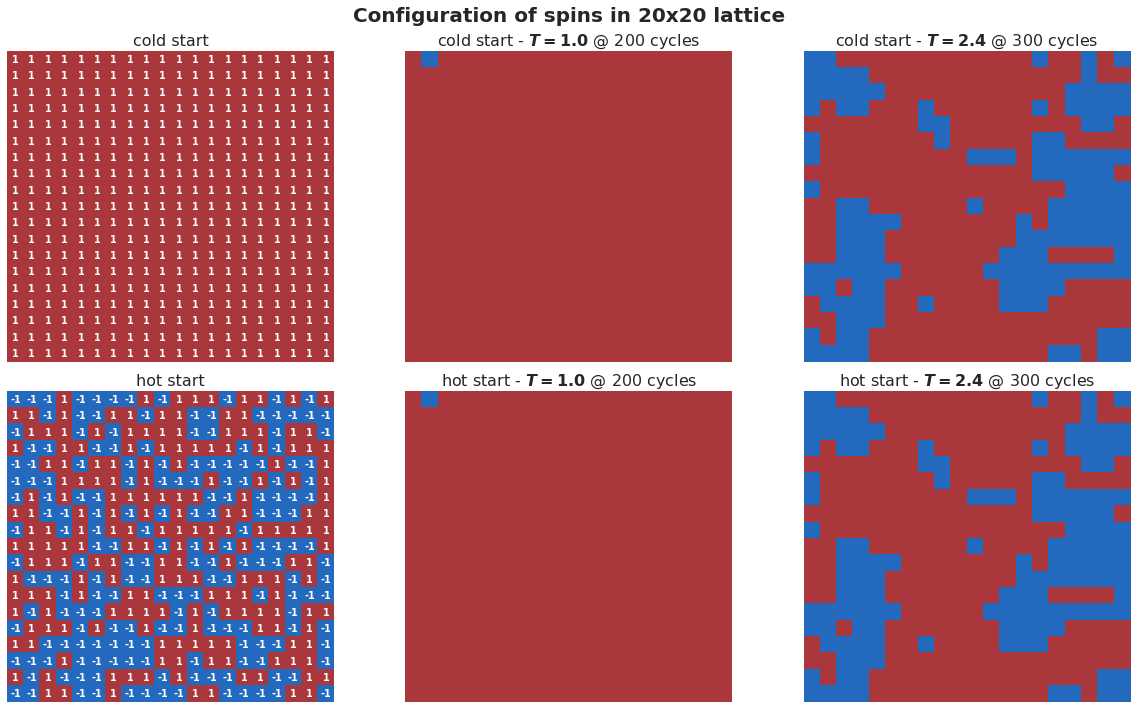
\includegraphics[width=1\linewidth]{./figs/20x20-config-spins.png}
	\caption{Configuration of spins in a $20 \times 20$ lattice at the start of the process to the left ($T=0$ in the upper and $T \rightarrow \infty$ in the lower). In the middle and to the right we see that after the confluence of the hot and cold trajectories in Figure \ref{fig:20x20-flips-per-cycle}, the evolution is independent of the starting conditions.}
	\label{fig:20x20-config-spins}
\end{figure}

\subsection{Approximation of the Energy Probability Distribution} \label{sec:prob-dist}
The energy probability distribution $P(E)$ gives the aggregated likelihood of having a lattice configuration with discrete energy $E_i$. Finding this analytically would require that we sum the configuration probability of all lattice configurations corresponding to $E_i$. Approximating the energy distribution, on the other hand, involves only that we sample the configuration energies and sort them from lowest to highest. 

Figure \ref{fig:20x20-prob-dist} shows the probability distributions at temperatures $T = 1.0$ $J/k_B$ and $T = 2.4$ $J/k_B$ for our $20 \times 20$ lattice. We have sampled the energy after every Monte Carlo cycle for $10^4$, $10^5$ and $10^6$ cycles, and have allowed $10^3$ cycles for the equilibration of the model. Note the different scales on the $x$ axes. 

As expected from the discussion in the previous section, the distribution is concentrated to the left at lower temperatures, with only about one in one hundred cycles having a single down spin and one in one thousand having three. We see that increasing the temperature shifts the distribution to higher energies and also makes it broader. This is reflected in the higher variance of approximately 8.2, which is around 0.025 for the low temperature in the best estimate, and corresponds well to our Figures \ref{fig:20x20-config-energy}, \ref{fig:20x20-flips-per-cycle} and \ref{fig:20x20-config-spins}. The expectation value at $T = 2.4$ $J/k_B$ is $\mathbb{E}(E) \approx 1.20$, which also corresponds well to our result in the previous section.

\begin{figure}[!h]
	\centering
	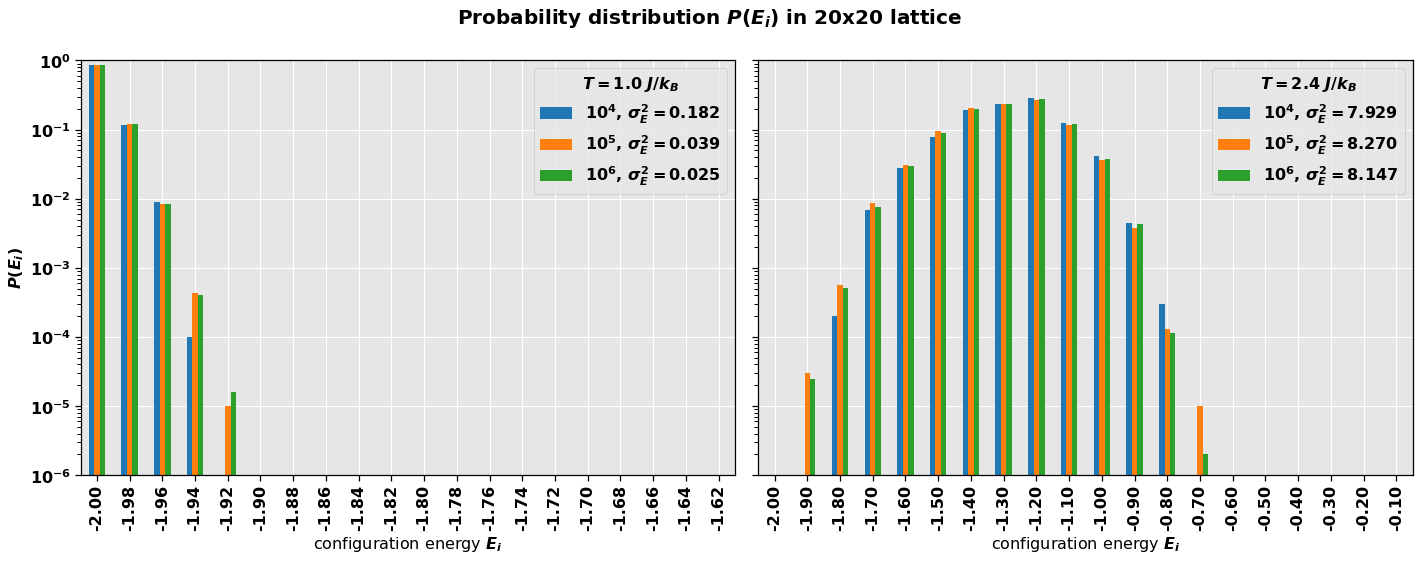
\includegraphics[width=1\linewidth]{./figs/20x20-prob-dist.png}
	\caption{Energy probability distribution for a $20 \times 20$ lattice at temperatures $T = 1.0$ $J/k_B$ and $T = 2.4$ $J/k_B$. Note the logarithmic scale. At low temperature, the distribution is heavily concentrated at the lower energies. For higher temperatures, the distribution is shifted to higher energies and is much broader. This corresponds well to the change in variance.}
	\label{fig:20x20-prob-dist}
\end{figure}

\subsection{Finding the Phase Transitions} \label{sec:phase-trans}
We have seen that at low temperatures, all or almost all spins are aligned up, and as temperature in the lattice increases, scattered areas of downs appear. See Figure \ref{fig:20x20-config-spins}. In an infinite lattice, this process reaches a critical temperature $T_C$, where $\mathbb{E}(\mathcal{M})$ abruptly goes to zero. Any increase beyond this temperature makes the scattered areas of up and down spins smaller until $T \rightarrow \infty$, where complete randomness prevails.

Our simulation model must have finite extension to be of any use to us, but we will not observe the same abrupt changes in mean magnetization. The critical temperature is still visible to us, especially in the heat capacity, but it is shifted to a higher temperature. See Figure \ref{fig:2x2-mum-cv}, where we have plotted the analytical mean magnetic moment and heat capacity for a $2 \times 2$ lattice using Equations (\ref{eq:energy-analytical}) and (\ref{eq:moment-analytical}). 

\begin{figure}[!h]
	\centering
	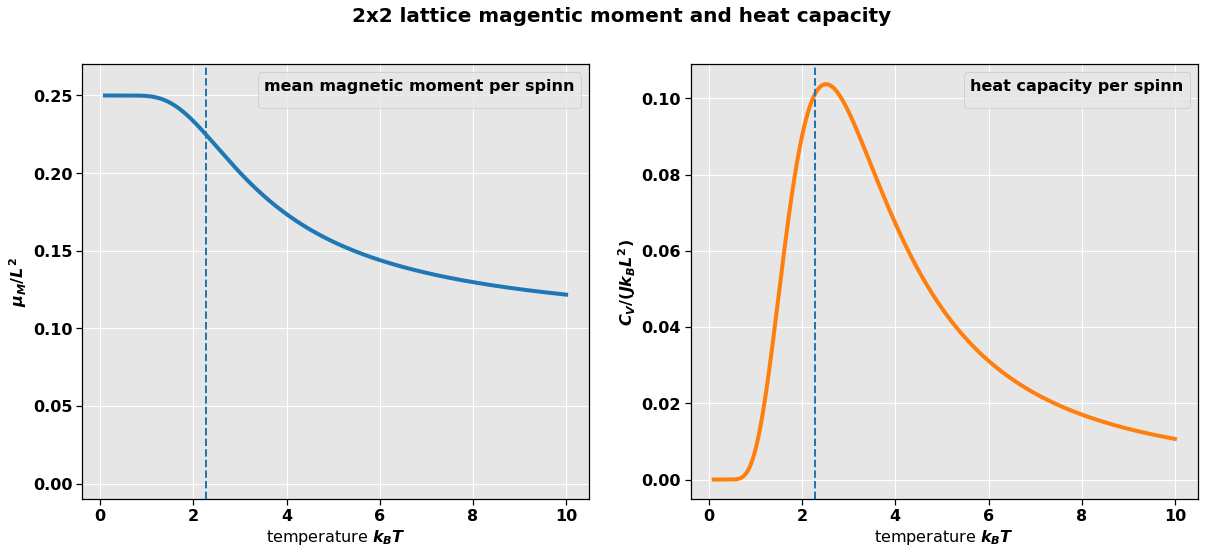
\includegraphics[width=1\linewidth]{./figs/2x2-mum-cv.png}
	\caption{Plots of the analytical magnetic moment expectation value and heat capacity for a $2 \times 2$ lattice as a function of $T$. The critical temperature $T_C \approx 2.269$ $J/k_B$ of the infinite lattice is indicated by the vertical dotted line. The critical temperature is shifted to a higher temperature for any finite lattice.}
	\label{fig:2x2-mum-cv}
\end{figure}

The critical temperature $T_C^{(\infty)}$ of the infinite lattice is indicated by the vertical line, while the critical temperature $T_C^{(2 \times 2)}$ occurs at the maximum value of the heat capacity. The relation between the critical temperatures of the finite and the infinite lattices are given by
\begin{equation}
	T_C^{(L \times L)} - T_C^{(\infty)} = \frac{\alpha}{L},
\end{equation}
where $\alpha$ is an unknown constant and $L$ is the lattice size. See \cite{fys4150-p4}. By running simulations with two lattice sizes $L_1, L_2$, we find the infinite lattice critical temperature;
\begin{equation}
	T_C^{(\infty)} = \frac{L_1 T_C^{(L_1 \times L_1)} - L_2 T_C^{(L_2 \times L_2)}}{L_1 - L_2}.
\end{equation}

Figure \ref{fig:temp-range-all} shows plots of the approximated properties for lattice sizes $L=40$, 60, 80 and 100. We have made two runs for each lattice size. First once over a wide range $T \in [2.0, 2.35]$ with step size $\Delta T = 0.05$ and $1 \times 10^5$ samples at each step. Then in a narrower range $T \in [2.25, 2.35]$ steps $\Delta T = 0.01$ and $2 \times 10^5$ samples to get a finer precision. 

In the upper right pane we see that the mean magnetic moment drops off sharper for increased lattice size, corresponding well with what we would expect. We also see that the peak in the heat capacities and susceptibilities seem to move left towards $T_C^{(\infty)}$, which again is indicated by the vertical line. The expected tendency is that larger $L$ should move the peak closer to $T_C^{(\infty)}$, but from the results in this figure, that is not clear.

For the $80 \times 80$ and $100 \times 100$ lattices. the peaks seem to lay in the [2.27, 2.29] range. We narrow our search further to only include these two lattices, and run simulations at each step $\Delta T = 0.002$ with $1 \times 10^6$ samples. 

The results are shown in Figure \ref{fig:temp-range-unall}. Still, the curves do not show a smooth development, fluctuating up to 5-6 \% for the $100 \times 100$ lattice. But picking the maximum values gives a fairly good estimate
\begin{equation}
	T_C^{(\infty)} \approx \frac{100 \cdot 2.278 - 80 \cdot 2.282}{100 - 80} = 2.262,
\end{equation}
which deviates about 0.31 \% from the analytical value $T_C^{(\infty)} = 2/\ln (1 + \sqrt{2}) \approx 2.269$ $J/k_B$ \cite{fys4150-p4}.

\begin{figure}[!h]
	\centering
	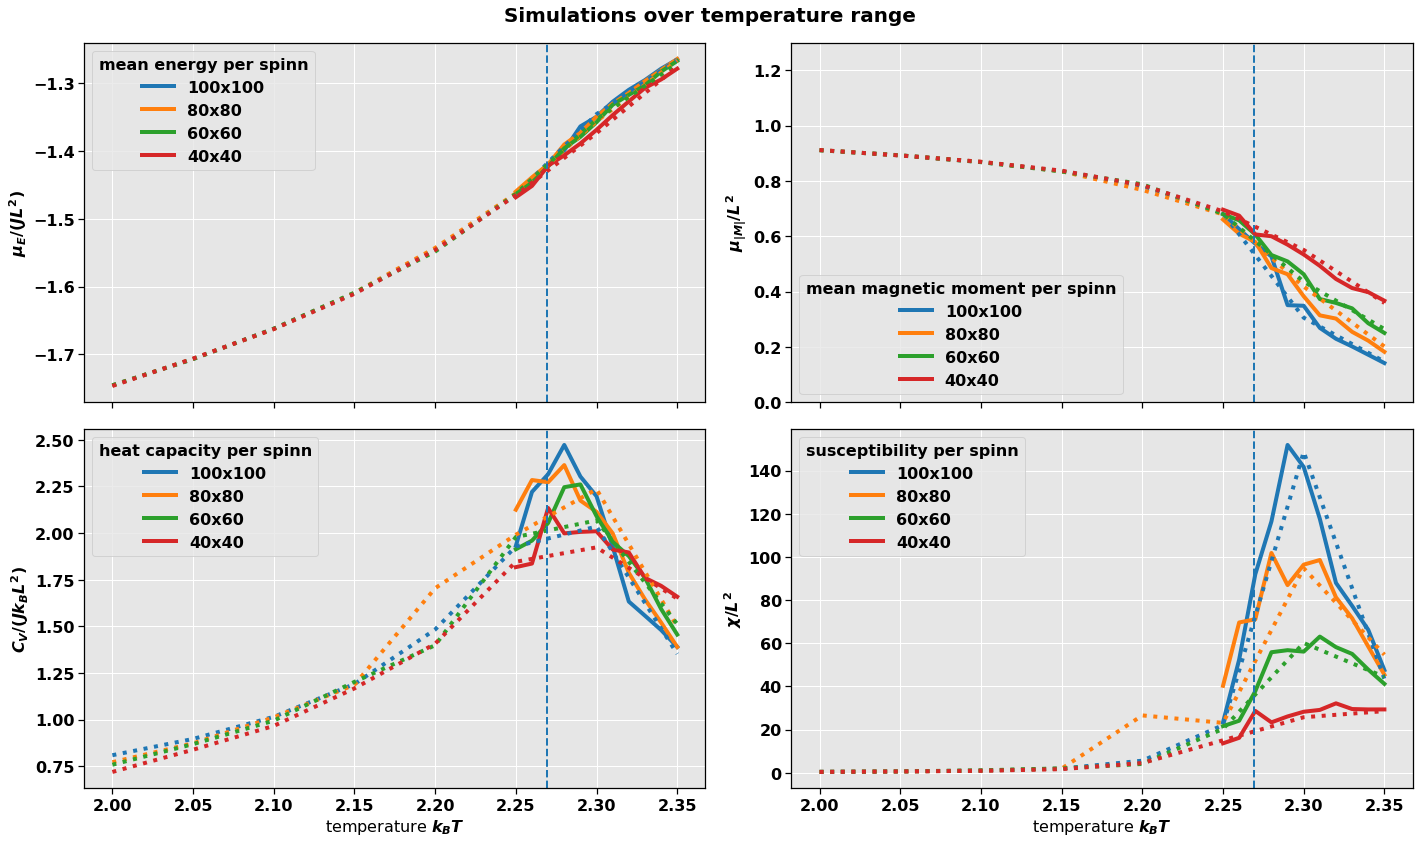
\includegraphics[width=1\linewidth]{./figs/temp-range-all.png}
	\caption{Simulations over temperature range with different lattice sizes. The dotted lines indicate the first run with lower sampling, and the full lines the second run with higher sampling. The critical temperature for each lattice $T_C^{(L \times L)}$ are best visible as the peaks in the heat capacities and susceptibilities (bottom panes).}
	\label{fig:temp-range-all}
\end{figure}


\begin{figure}[!h]
	\centering
	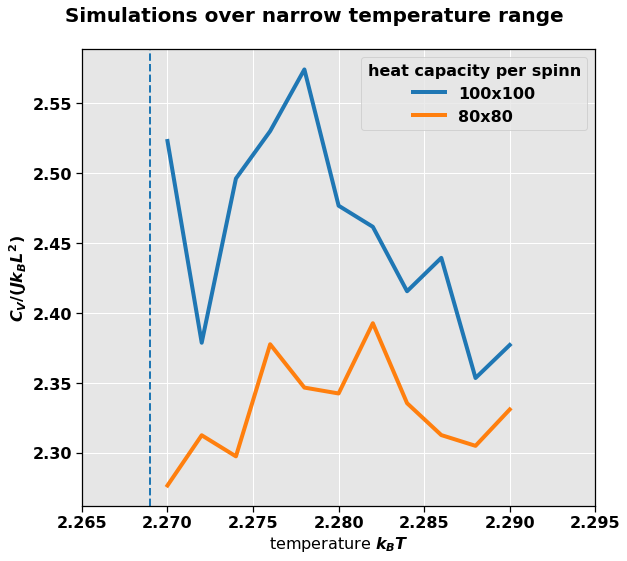
\includegraphics[width=.5\linewidth]{./figs/temp-range-unall.png}
	\caption{Narrowed search for the critical temperature with finer steps and higher sampling than in Figure \ref{fig:temp-range-all}. Still, the heat capacity estimates do not have a smooth development, but the approximation of $T_C^{(\infty)}$ deviates only 0.31 \% from the analytical value.}
	\label{fig:temp-range-unall}
\end{figure}

\clearpage
\section{Discussion and Conclusion} \label{sec:conclusion}
% - State your main findings and interpretations
% - Try as far as possible to present perspectives for future work
% - Try to discuss the pros and cons of the methods and possible improvements

We have shown that the two-dimensional Ising model can be interpreted as a reversible Markov process. We have used Monte Carlo simulations with the Metropolis algorithm as acceptance criteria for evolving the process, and seen that it converges towards its most likely state, independently of the initial conditions. As such, the initial conditions can be selected freely, but the equilibration time will depend on our selection at least to some degree.

We have seen that the configuration of spins starts with almost all being in the up state at low temperatures, and that increasing temperature leads to higher number of downs. We have also seen that the ups and downs tend to form patches, corresponding well to the spins' preference of attaining the same state as their nearest neighbors.

Monte Carlo simulation can also be used to approximate the discrete probability distribution of the lattice energy, $P(E)$. The distribution is heavily weighted towards the lower energy limit $-2J$ per spin at lower temperatures, and moves to higher energies as temperature increases. We have seen that this corresponds to increased variance, meaning that the distribution broadens. This is a consequence of the increased kinetic energy which means that more energy states are likely to occur. The higher energy limit of the lattice is $+2J$ per spin, but $\mathbb{E}(E)$ will never move above 0, since that corresponds to $T \rightarrow \infty$.

For a small lattice of $2 \times 2$ spins, where analytical expressions are easily attained, we have shown that our model approximates the magnetic energy and moment expectation value and variance with high precision, but that this requires $> 10^6$ Monte Carlo cycles. Proofing our model on the $2 \times 2$ lattice had the added benefit of putting our model to the test with regards to the correct assumptions concerning the Metropolis algorithm, and the implementation of boundary values, since all spins are one the edge of the lattice.

Finally, we have shown that our model correctly reproduces the critical temperature, which in an infinite lattice leads to phase transition (the magnetic moment goes abruptly to zero). Based on our simulations, we estimated the analytical critical temperature with an error of 0.31  \%.

\vspace{5mm}

As an extension of the study done in this report, it would be interesting to look at how the Ising model could be used in other settings. Many phenomena present themselves as scattered continuous areas of equal orientation. These may be the formation of cracks and weaknesses in a structure or the spread of a decease in a population. Further insight into the Ising model, by tuning of the coupling $J$ or extension into higher dimensions could help solve such problems.

%\clearpage
\bibliographystyle{unsrt}
\bibliography{project4.bib}
\end{document}
